\begin{frame}{Tangential Node Shifting -- Neck}
    \centering
    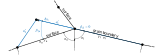
\includegraphics[width=\linewidth]{img/model_development/node_shift_tangential_neck}
    \begin{columns}
        \begin{column}{0.5\linewidth}
            \begin{equation*}
                \frac{\partial \GibbsEnergy}{\partial {\Shift}_{\Tangential}} = -\left( {\InterfaceEnergy}_{\Upper} \cos \SurfaceVectorAngle_{\Tangential\Upper} - {\InterfaceEnergy}_{\Lower} \cos \SurfaceVectorAngle_{\Tangential\Lower}\right)
            \end{equation*}
        \end{column}
        \begin{column}{0.5\linewidth}
            \begin{equation*}
                \frac{\partial \Volume}{\partial {\Shift}_{\Tangential}} = \frac{1}{2} \left( \SurfaceDistance_{\Upper} \sin \SurfaceVectorAngle_{\Tangential\Upper} - \SurfaceDistance_{\Lower} \sin \SurfaceVectorAngle_{\Tangential\Lower}\right)
            \end{equation*}
        \end{column}
    \end{columns}
\end{frame}
